% document formatting
\documentclass[10pt]{article}
% \usepackage[UTF8]{inputenc}
\usepackage[UTF8, scheme=plain]{ctex}
\usepackage[left=1in,right=1in,top=1in,bottom=1in]{geometry}
\usepackage[T1]{fontenc}
\usepackage{xcolor}

% math symbols, etc.
\usepackage{amsmath, amsfonts, amssymb, amsthm}

% lists
\usepackage{enumerate}
\usepackage[table,xcdraw]{xcolor}

% images
\usepackage{graphicx} % for images
\usepackage{tikz}

% code blocks
% \usepackage{minted, listings} 

% verbatim greek
\usepackage{alphabeta}

\graphicspath{{./assets/images/Week 1}}

\title{02-741 Week 1 \\ \large{Generative AI for Biomedicine}}
 
\author{Aidan Jan}

\date{\today}

\begin{document}
\maketitle

\section*{Introduction to Molecular and Cell Biology}
We don't quite understand ourselves.  In the human body, there are tens of trillions of cells, and dozens of different cell types.  (Just neurons have over ten different types.)  However, we do not understand how cells differentiate.  For example, why a muscle cell originally grew into a muscle cell, or why a neuron originally grew into a neuron.  Additionally, we don't know how to change one cell type into another cell type.  (e.g., Skin cell $\rightarrow$ Stem cell $\rightarrow$ Neuron.)\\\\
One domain of current research is with gene expression.  Since all cells have the same DNA, what features (or activation of genes) would cause a stem cell to become a certain cell type?  Given some information on which genes are activated, can we predict what cell type the cell is?  This is where AI comes in.

\subsection*{Decoding the ``Language'' of Genomes, Cells, and Tissues}
Biology is multi-scale.  We can observe gene sequences, cell structure, and cell function, all of which are at different scales.  As a result, our models must also be multi-scale.

\subsection*{Central Dogma of Biology}
Proteins do most of the work in biology, and are encoded by subsequences of DNA, known as genes.
\begin{center}
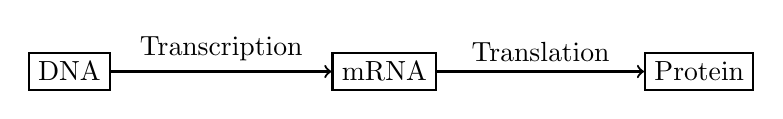
\begin{tikzpicture}
    \node[draw, thick] at (0, 0) (a) {DNA};
    \node[draw, thick] at (4, 0) (b) {mRNA};
    \node[draw, thick] at (8, 0) (c) {Protein};

    \draw[->, thick] (a) -- node[above] {Transcription} (b);
    \draw[->, thick] (b) -- node[above] {Translation} (c);
\end{tikzpicture}
\end{center}

\subsection*{The Human Genome: the ``Blueprint'' of Our Body}
\begin{itemize}
    \item $10^{13}$ different cells in an adult human
    \item The cell is the basic unit of life
    \item DNA = linear molecule inside the cell that carries instructions needed throughout the cell's life - long string(s) over a small alphabet
    \item Alphabet of four nucleotides / bases.  (A, C, T, G)
\end{itemize}
DNA organizes into chromatin, which form into nucleosomes, which condenses into chromosomes.  Humans have 22 pairs of chromosomes, plus the two sex chromosomes.

\subsection*{Genomes}
\begin{itemize}
    \item A genome is an organism's complete set of DNA (including its genes)
    \item In humans, less than 2\% of the genome actually encodes for genes
    \item However, a much larger percentage of the genome is transcribed (miRNAs, IncRNAs, and other non-coding RNAs\dots)
    \item \dots and a large fraction of the rest of the genome serves as control regions, i.e., these regions are involved in determining when genes are turned on and off depending on the context.
\end{itemize}

\subsection*{Structure of Genes in Mammalian Cells}
\begin{itemize}
	\item Within coding DNA genes there can be untranslated regions (\textbf{introns})
	\item The translated parts are termed \textbf{exons}.  These are the segments of DNA that contain the protein coding information.
	\item Following transcription, introns are removed and exons are \textbf{spliced} to make the \textbf{protein}.
	\item \textbf{Alternative splicing} increases the potential number of different proteins, allowing the generation of millions of proteins from a small number of genes.
\end{itemize}

In recent years (2001 - Present), high throughput DNA sequencing allows for cheap sequencing of human DNA.  In 2001, one genome costs over \$100,000,000.  Now (2026), it costs less than \$800 per genome.  High-throughput DNA sequencing is one of the most disruptive technologies in the past decade.

\subsubsection*{Understanding the Genome}
\begin{itemize}
    \item View from 2000
    \begin{itemize}
        \item Protein coding regions: 35000-120000
        \item Regulatory sequence: Less than protein-coding information
        \item Transposons: Junk DNA
        \item (All of these assumptions are wrong!)
    \end{itemize}
    \item We now know\dots
    \begin{itemize}
        \item Protein coding regions: 20000.  (Fewer than fish!)
        \item Regulatory sequences: More regulatory sequences than protein-coding regions
        \item Transposons: Make up half of the human genome
        \item Gene numbers do not correlate with organism complexity
        \item 5\% of genes are conserved between different species, but only 1.5\% actually codes for proteins
    \end{itemize}
\end{itemize}

\subsubsection*{The Spectrum of Genetic Variation}
\begin{tabular}{|l|l|l|}
\hline
\rowcolor[HTML]{FFCE93} 
\textbf{Variation}                                                                & \textbf{Rearrangement type}                                                                                                                                         & \textbf{Size range}                                                         \\ \hline
Single base-pair changes                                                          & \begin{tabular}[c]{@{}l@{}}Single nucleotide polymorphisms (SNPs), \\ point mutations\end{tabular}                                                                  & 1 bp                                                                        \\ \hline
Small insertions / deletions                                                      & \begin{tabular}[c]{@{}l@{}}Binary insertion/deletion events of short\\ sequences (majority \textless{}10 bp in size)\end{tabular}                                   & 1-50 bp                                                                     \\ \hline
Short tandem repeats                                                              & Microsatellites and other simple repeats                                                                                                                            & 1-500 bp                                                                    \\ \hline
Fine-scale structural variation                                                   & \begin{tabular}[c]{@{}l@{}}Deletions, duplications, tandem repeats,\\ inversions\end{tabular}                                                                       & 50 bp to 5 kb                                                               \\ \hline
Retroelement insertions                                                           & SINEs, LINEs, LTRs, ERVs                                                                                                                                            & 300 bp to 10 kb                                                             \\ \hline
\begin{tabular}[c]{@{}l@{}}Intermediate-scale structural\\ variation\end{tabular} & \begin{tabular}[c]{@{}l@{}}Deletions, duplications, tandem repeats,\\ inversions\end{tabular}                                                                       & 5 kb to 50 kb                                                               \\ \hline
Large-scale structural variation                                                  & \begin{tabular}[c]{@{}l@{}}Deletions, duplications, large tandem repeats,\\ inversions\end{tabular}                                                                 & 50 kb to 5 Mb                                                               \\ \hline
Chromosomal variation                                                             & \begin{tabular}[c]{@{}l@{}}Euchromatic variants, large cytogenetically\\ visible deletions, duplications, translocations,\\ inversions, and aneuploidy\end{tabular} & \begin{tabular}[c]{@{}l@{}}$\sim$5 Mb to entire \\ chromosomes\end{tabular} \\ \hline
\end{tabular}

\subsection*{Transcriptional Regulation}
\begin{center} 
	\includegraphics*[width=\textwidth]{W1_10.png} 
\end{center}
\begin{itemize}
	\item Transcription start site (TSS)
	\item Transcription factor binding sites (TFBS)
	\item Cis-regulatory module (CRM)
	\item Proximal promoter and distal enhancer
\end{itemize}

\subsection*{Transcription Factors (TFs) in the Human Genome}
\begin{itemize}
	\item 300 TFs bind to core promoter regions
	\begin{itemize}
	    \item General transcription machinery (e.g., RNA polymerase)
	    \item Required for transcription of most protein-coding genes
    \end{itemize}
    \item 1500 TFs bind to other regions in the genome
    \begin{itemize}
	    \item Proximal promoter, enhancer, silencer
	    \item Regulate a subset of genes
    \end{itemize}
\end{itemize}

\subsection*{How is Specificity of Binding Achieved?}
\begin{itemize}
	\item Consensus motif
	\begin{itemize}
	    \item Commonly found sequence
	    \item Shows which nucleotide is most abundant at each position, represented as a Position Weight Matrix (PWM)
	    \item E.g., GATA1 binding motif: [AT] GATA [AG]
    \end{itemize}
    \item Motif: A subsequence (substring) that occurs in multiple sequences with a biological importance
    \item Motifs can be totally constant or have variable elements
    \item Motifs for regulatory elements
    \begin{itemize}
	    \item Binding sites for proteins
	    \item Short sequences (5-25 bp)
	    \item Up to a certain range, e.g., 1000 bp (or farther), from gene
	    \item Inexactly repeating patterns (challenge!)
    \end{itemize}
\end{itemize}

\subsection*{From One Cell to Trillions}
\begin{itemize}
	\item Humans have multiple types of cells
	\item Individual cell types also differentiate into sub-cell types
	\item Lots more cell types left to discover!
\end{itemize}

\subsection*{DNA is Only Half the Story}
\begin{itemize}
	\item Variations in DNA alone may not entirely account for variations in phenotypic traits.
	\item Organisms with identical DNA often exhibit distinct phenotypes
	\begin{itemize}
	    \item Includes plants, insects, mammals, etc.
    \end{itemize}
\end{itemize}

\subsection*{What is Epigenetics / Epigenomics?}
\begin{itemize}
	\item A mitotically or meiotically heritable state of different gene activity and expression (\textbf{phenotype}) that is independent of differences in DNA sequence (\textbf{genotype})
	\begin{itemize}
	    \item - based on Conrad Waddington, 1942
    \end{itemize}
	\item The sum of the alterations to the chromatin template that collectively establish and propagate different patterns of gene expression (transcription) and silencing from the same genome.
    \item Epigenetic changes influence the phenotype without altering the genotype.
    \item While \textbf{epigenetics} often refers to the study of single genes or sets of genes, \textbf{epigenomics} refers to more global analyses of epigenetic changes across the entire genome.
\end{itemize}

\subsection*{Epigenetic Mechanisms}
\begin{itemize}
	\item DNA Methylation
	\begin{itemize}
	    \item Normal cells - role in gene expression and chromosome stability
	    \item Cancer cells - consequences of aberrant hypo- and hyper-methylation
    \end{itemize}
	\item Histone Modification
	\begin{itemize}
	    \item Normal cells - the histone code
	    \item Cancer cells - consequences of altered histone modifying enzymes
    \end{itemize}
	\item Interaction between DNA methylation, histone modifications, and other players such as non-coding RNAs
	\item Cell and tissue type specificity
	\item Gene-environment interaction, disease susceptibility
\end{itemize}
If DNA is like the alphabet, epigenetic marks are like the accents and punctuation.  If DNA is like a book, epigenetic marks are like sticky notes.

\subsection*{Chromatin Structures}
\begin{itemize}
	\item Eukaryotic chromatin structure can be viewed as a series of superimposed organizational layers.     
    \item At the root are the DNA sequence and its direct chemical modification by \textbf{cytosine methylation}.     
    \item The DNA is folded into \textbf{nucleosomes} — the fundamental units of chromatin — that comprise approximately 147 bp of DNA wrapped around a histone octamer.     
    \item The nucleosomal \textbf{histones} H2A, H2B, H3 and H4 can be chemically modified and exchanged with variants. The nucleosome positions along with histone variants and modifications make up the primary structure of chromatin.     
    \item Finally, three-dimensional models of chromatin in nuclei are now being developed with increasing precision and propose that there are additional sophisticated layers of genome regulation through \textbf{higher-order organization} and \textbf{nuclear compartmentalization}.
\end{itemize}

\subsection*{Higher-Order Genome Organization}
\begin{itemize}
	\item We can now determine a genome's sequence and annotate linear chromatin composition, but our genome is not linear
    \item Our knowledge of the 3D organization of the genome remains limited
    \item Need to achieve high spatial and temporal resolution
\end{itemize}

\section*{Sequence Modeling and Generation with Transformer}
Can we use GenAI to design molecules with desired functions?
\begin{itemize}
	\item Medicine
	\item Vaccines
	\item Enzymes (Biocatalysts)
	\item Biosensors (e.g., GFP)
	\item New materials
\end{itemize}
Molecule generation is somewhat similar to language generation.
\begin{itemize}
	\item Both are sequences of discrete tokens.  (In language it's words, in molecules, it is atoms or amino acids.)
	\item Both have discrete structures.  (In language it's grammar, in molecules it's chemistry)
	\item Geometry (Unique for molecules)
\end{itemize}
For proteins, they can be roughly represented as sequences of amino acids.
\begin{itemize}
	\item Proteins are building blocks of life
	\item Responsible for important biological functions
	\item Built by sequences of amino acids.
	\begin{itemize}
	    \item GFP (Green Fluorescent Protein) = VLLPDNHYLSTQSALSKDPNEKRDHMVLLEFVTAAGIT
    \end{itemize}
\end{itemize}

\section*{Language Models}
A language model is a probabilistic model of discrete sequences, including human languages and biological languages.  e.g.,
\begin{align*}
    &\text{Probability}(\text{``Pittsburgh is a city of bridges''})\\
    &\text{Probability}(\text{``VLLPDNHYLSTQSALSKDPNEKRDHMVLLEFVTAAGIT''})
\end{align*}
Each next token can be defined as a probability based on previous tokens.
\[P(\text{next word } y_t | \text{Prompt } x, \text{previous words } y_{1\::\: t - 1})\]
For example,
\begin{itemize}
	\item Santa Barbara has very nice \underline{\hspace{2cm}}
	\begin{itemize}
	    \item ``beach'' = 0.5 
	    \item ``weather'' = 0.4
	    \item ``snow'' = 0.01
    \end{itemize}
    \item Pittsburgh is a city of \underline{\hspace{2cm}}
    \begin{itemize}
	    \item ``bridges'' = 0.6
	    \item ``corn'' = 0.02
    \end{itemize}
\end{itemize}
To calculate the probabilities, the probability of each word (or each amino acid) depends on all the previous tokens.
\begin{align*}
    &P(\text{``Pittsburgh is a city of bridges''}) \\
    &= P(\text{``Pittsburgh''}) \cdot P(\text{``is''} | \text{``Pittsburgh''}) \cdot P(\text{``a''} | \text{``Pittsburgh is''}) \cdot P(\text{``city''} | \dots) \\
    &\cdot P(\text{``of''} | \dots) \cdot P(\text{``bridges''} | \dots)
\end{align*}
Or simply,
\[P(x_{1\dots T}) = \prod_{t = 1}^T P(x_{t + 1} | x_{1\dots t})\]
We can predict the $P(x_{t + 1} | x_{1 \dots t})$ part using neural networks (e.g., CNNs, RNNs)

\subsection*{Types of Language Models}
\begin{itemize}
	\item \textbf{Encoder-only Model} (or Masked LM, Non-autoregressive)
	\begin{itemize}
	    \item Examples: BERT, RoBERTa, ESM (for protein)
    \end{itemize}
    \item \textbf{Encoder-decoder}
    \begin{itemize}
	    \item Example: T5
    \end{itemize}
    \item \textbf{Decoder-only} (Autoregressive)
    \begin{itemize}
	    \item Examples: GPT, LLaMA, ProGen (for proteins)
    \end{itemize}
\end{itemize}

\subsection*{Encoder-Decoder Paradigm}
\begin{center}
\begin{tikzpicture}
    \node[draw, rectangle, thick] at (0, 0) (e) {Encoder};
    \node[draw, rectangle, thick] at (6, 0) (d) {Decoder};

    \draw[->] (e) -- (d);
    \node at (0, -0.5) (e_) {Input: 我喜欢唱歌和跳舞。};
    \node at (6, -0.5) (d_) {Target: I like singing and dancing.};
\end{tikzpicture}
\end{center}

\subsection*{Sequence to Sequence Learning}
\begin{itemize}
	\item Conditional text generation: directly learning a function mapping from source sequence to target sequence
	\[p_\theta(y | x) = \prod_t p(y_t | x, y_{1: t - 1}; \theta)\]
    \item Previous encoder / decoder: LSTM or GRU
\end{itemize}
\begin{center} 
	\includegraphics*[width=\textwidth]{W1_1.png} 
\end{center}
We use the encoder-decoder architecture because it is
\begin{itemize}
	\item Full context and parallel: use Attention in both encoder and decoder
	\item Not recurrent $\Rightarrow$ concurrent encoding
\end{itemize}

\subsection*{Motivation of Attention: Translation between Different Alignment of Words}
\begin{center} 
	\includegraphics*[width=\textwidth]{W1_2.png} 
\end{center}
Different languages have different orderings for words.

\subsection*{Transformer-based Models for Biomolecules}
\begin{itemize}
	\item Protein Language Models:
	\begin{itemize}
	    \item ESM, ESM-Fold
	    \item ProGen
	    \item AlphaFold (with EvoFormer)
    \end{itemize}
    \item Genomics
    \begin{itemize}
	    \item DNABERT / DNABERT2
	    \item Evo, Evo2
	    \item ENABERT
    \end{itemize}
    \item Single Cell: scGPT, scFoundation
\end{itemize}

\section*{Transformers}
\begin{center} 
	\includegraphics*[width=\textwidth]{W1_3.png} 
\end{center}
What is Embedding?
\begin{itemize}
	\item Token Embedding: 
	\begin{itemize}
	    \item token index $\rightarrow$ vector
	    \item Shared (tied) input and output embedding from lookup table
    \end{itemize}
    \item Positional Embedding
    \begin{itemize}
	    \item to distinguish words in different positions, map position labels to embedding, dimension is same as token embedding
	    \item For $t$-th position, $i$-th dimension, the equation is:
    \end{itemize}
    \begin{align*}
        PE_{t, 2i} &= \sin \left(\frac{t}{1000^{2i / d}}\right) \\
        PE_{t, 2i + 1} &= \cos \left(\frac{t}{1000^{2i / d}}\right)
    \end{align*}
\end{itemize}
\begin{center} 
	\includegraphics*[width=0.6\textwidth]{W1_4.png} 
\end{center}

\subsection*{Multi-head Attention}
\begin{itemize}
	\item Instead of one vector for each token, we break it into multiple heads
	\item Each head performs attention.
\end{itemize}
\begin{align*}
    \text{Head}_i &= \text{Attention}(QW_i^Q, KW_i^K, VW_i^V) \text{MultiHead}(Q, K, V) \\
    &= \text{Concat}(\text{Head}_1, \text{Head}_2, \dots, \text{Head}_h) W^O
\end{align*}
\begin{center} 
	\includegraphics*[width=\textwidth]{W1_5.png} 
\end{center}
The $\sqrt{d_k}$ is a regularization coefficient, where $d_k$ is the dimensionality of the attention (number of heads).  This coefficient makes it softmax is a range from 0 to 1.

\subsubsection*{Multihead Attention and FFN}
\begin{align*}
    \text{Attention}(Q, K, V, x) &= \text{Softmax}\left(\frac{(Qx)^T Kx}{\sqrt{d}}\right) \cdot (Vx)^T \\
    \text{FFN}(x) &= max(0, x \cdot W_1 + b_1)\cdot W_2 + b_2
\end{align*}
\begin{center} 
	\includegraphics*[width=0.7\textwidth]{W1_6.png} 
\end{center}

\subsubsection*{Attention Variant: Grouped-Query Attention (GQA)}
\begin{align*}
    \text{Head}_i = \text{Attention}(XW_h^Q, XW_{g(h)}^K, XW_{g(h)}^V) \\
    \text{MultiHead}(Q, K, V) = \text{Concat}(\text{Head}_1, \text{Head}_2, \dots, \text{Head}_h)W^O
\end{align*}
\begin{center} 
	\includegraphics*[width=0.9\textwidth]{W1_7.png} 
\end{center}
Grouping the queries can speed up the inference since there are less overall matrix multiplications.

\subsubsection*{Attention Variant: Multi-head Latent Attention (MLA)}
\begin{itemize}
	\item Keys and values occupy large GPU memory
	\begin{itemize}
	    \item $2 \cdot len \cdot n_h \cdot d_h$
    \end{itemize}
    \item instead of caching $d_h$ vector (for each $t_k$, head), reduce to a latent space with rank $r$.
    \begin{center} 
	    \includegraphics*{W1_8.png} 
    \end{center}    
    \item First proposed in Deepseek-V2, used in all modern LLMs
    \item Key and Value share down-projection, and across all heads
\end{itemize}
\begin{align*}
&MLA(x)_h\\
&= \text{Softmax}\left(\frac{X \cdot W_Q^D \cdot W_{Q, h}^U \cdot \left(X \cdot W_{KV}^D \cdot W_{K, h}^U\right)^T}{\sqrt{d_h}}\right)\cdot X \cdot W_{KV}^D \cdot W_{V, h}^U \\
&= \text{Softmax}\left(\frac{C_Q \cdot W_{QK, h} \cdot C_{KV}^T}{\sqrt{d_h}}\right) \cdot C_{KV} \cdot W_{V, h}^U
\end{align*}
We can precompute and cache the following:
\begin{align*}
    W_{QK, h} &= W_{Q, h}^U \cdot (W_{K, h}^U)^T \\
    C_Q &= X \cdot W_Q^D \\
    C_{KV} &= X \cdot W_{KV}^D
\end{align*}

\subsection*{Decoder Self-Attention Mask}
\begin{itemize}
	\item Encoder uses bidirectional attention
	\item Decoder uses unidirectional attention
	\begin{itemize}
	    \item Maskout right side before softmax (-inf)
        \begin{center} 
	        \includegraphics*[width=0.4\textwidth]{W1_9.png} 
        \end{center}
    \end{itemize}
\end{itemize}

\newpage
\subsection*{FFN with SwiGLU}
The swish activation function looks like
\begin{center} 
	\includegraphics*[width=0.5\textwidth]{W1_11.png} 
\end{center}
\[swish(x) = x\sigma(\beta x)\]
\[\sigma(x) = \frac{1}{1 + e^{-x}}\]
FFN with ReLU:
\[FFN(x) = max(0, x \cdot W_1 + b_1) \cdot W_2 + b_2\]
FFN with SwiGLU:
\[FFN_{SwiGLU}(x) = (swish(x \cdot W_1 + b_1) \odot (x \cdot W_2 + b_2)) \cdot W_3 + b_2\]
\begin{itemize}
	\item FFN with SwiGLU is used in LLaMA and all later LLMs.
\end{itemize}

\subsection*{Residual Connection and Layer Normalization}
\begin{itemize}
	\item Residual Connection
	\item Make it zero mean and unit variance within layer
	\item Post-norm
	\item Pre-norm
\end{itemize}
\begin{center} 
	\includegraphics*[width=0.45\textwidth]{W1_12.png} 
\end{center}

\subsection*{Relative Positional Embedding}
\begin{itemize}
	\item ``I have a dream''
	\item ``Today I have a dream''
\end{itemize}
What are Attention weights for ``I'' and ``dream''?  The goal is to make sure the similarity is only dependent on the distance between two embeddings, independent of their absolute positions
\[Att(x_i, x_j) = Att(x_{i + \Delta}, x_{j + \Delta})\]

\subsection*{Rotary Embedding (RoPE)}
Makes the attention weight depending (only) on position distance
\[f(x_m, m) = \begin{pmatrix} \cos(m\theta) & -\sin(m\theta) \\ \sin(m\theta) & \cos(m\theta) \end{pmatrix} \begin{pmatrix} x_{m, 1} \\ x_{m, 2} \end{pmatrix}\]
\[f(x_m, m) \cdot f(x_n, n) = x_m^T R_{n - m} x_n\]
\begin{center} 
	\includegraphics*[width=0.9\textwidth]{W1_13.png} 
\end{center}

\subsection*{Sparse Attention}
Alternating dense and locally banded \textbf{sparse attention} patterns (GPT3)
\begin{center} 
	\includegraphics*[width=0.9\textwidth]{W1_14.png} 
\end{center}

\section*{Training Techniques and Performance of Transformer}
\subsection*{Training Transformer}
\[P(Y | X) = \prod P(y_t | y_{<t}, x)\]
\begin{itemize}
	\item Training loss: Cross-Entropy
	\[\ell = -\sum_n \sum_t \log f_\theta (x_n, y_{n, 1}, \dots, y_{n, t - 1})\]
    \item Teacher-forcing during training.
    \item Pretend to know ground truth for prefix.
\end{itemize}

\subsection*{Training Transformer for MT}
\begin{itemize}
	\item Dropout
	\begin{itemize}
	    \item Applied to before residual, and to embedding, pos emb.
	    \item $p = 0.1 \sim 0.3$
    \end{itemize}
	\item Label smoothing
	\begin{itemize}
	    \item $0.1$ probability assigned to non-truth
    \end{itemize}
	\item Vocabulary
	\begin{itemize}
	    \item En-De: 37K using BPE
	    \item En-Fr: 32k word-piece (similar to BPE)
    \end{itemize}
\end{itemize}

\subsubsection*{Label Smoothing}
\begin{itemize}
	\item Assume $y \in R^n$ is the one-hot encoding of label
	\item Approximating $0/1$ values with softmax is hard
	\item The smoothed version is 
    \[y_i = \begin{cases} 1 - \epsilon & \text{if belongs to class $i$}\\ \epsilon / (n - 1) & \text{otherwise} \end{cases}\]
    \begin{itemize}
	    \item We commonly use $\epsilon = 0.1$.
    \end{itemize}
\end{itemize}

\subsection*{Training Technique}
\begin{itemize}
	\item Batch
	\begin{itemize}
	    \item group by approximate sentence length
	    \item still need shufflingHardware
	    \item one machine with 8 GPUs (in 2017 paper)
	    \item base model: 100k steps (12 hours)
	    \item large model: 300k steps (3.5 days)
    \end{itemize}
	\item Adam Optimizer
	\begin{itemize}
	    \item increase learning rate during warmup, then decrease
	    \item $\eta = \frac{1}{\sqrt{d}} \min \left(\frac{1}{\sqrt{d}}, \frac{t}{\sqrt{t_0^3}}\right)$
    \end{itemize}
\end{itemize}

\subsubsection*{Adam Optimizer}
\begin{align*}
m_{t + 1} &= \beta_1 m_t - (1 - \beta_1) \nabla \ell(x_t)\\
v_{t + 1} &= \beta_2 v_t + (1 - \beta_2) (\nabla \ell(x_t))^2 \\
\intertext{Momentum:}
\hat{m}_{t + 1} &= \frac{m_{t + 1}}{1 - \beta_1^{t + 1}} \\
\intertext{Variance:}
\hat{v}_{t + 1} &= \frac{v_{t + 1}}{1 - \beta_2^{t + 1}} \\
\intertext{Parameter Update:}
x_{t + 1} &= x_t - \frac{\eta}{\sqrt{\hat{v}_{t + 1}} + \epsilon} \hat{m}_{t + 1}
\end{align*}

\subsubsection*{Other Parameter Optimizers}
\begin{itemize}
	\item AdamW (used in LLaMA)
	\begin{itemize}
	    \item Similar to Adap but update with weight decay
    \end{itemize}
    \item Muon (used in deepseek models)
    \begin{itemize}
	    \item Update 2D weight matrix using fast and orthogonal Newton-Schulz iterations.
    \end{itemize}
\end{itemize}

\subsection*{Model Average}
\begin{itemize}
	\item A single model obtained by averaging the last 5 checkpoints, which were written at 10-minute intervals (base)
	\item Decoding length: within source length + 50
\end{itemize}

\subsection*{Summary}
\begin{itemize}
    \item Key components in Transformer and LLM Architecture
    \begin{itemize}
        \item Positional Embedding (to distinguish tokens at different positions)
        \item Multihead attention
        \item Residual connection
        \item Layer norm
        \item FFN and SwishGLU
        \item RoPE
    \end{itemize}
    \item Training Technique:
    \begin{itemize}
        \item Dropout
        \item Label smoothing
        \item Optimization algorithm
    \end{itemize}
    \item Pretraining: Mask-labeled recovery of random spans and next token prediction
    \item Multitask supervised fine-tuning with instruction templates
    \begin{itemize}
        \item T5, InstructGPT
    \end{itemize}
\end{itemize}


\end{document}